\documentclass{beamer}

% Theme choice
\usetheme{CambridgeUS} % professional, clean look
\usecolortheme{default} % colors can be adjusted if desired

% Packages
\usepackage[utf8]{inputenc}
\usepackage{graphicx}   % for including graphics
\usepackage{booktabs}   % for tables
\usepackage{amsmath, amssymb} % for math
\usepackage{hyperref}   % for clickable links

% Title page info
\title[]{Presentation of 'Employer Consolidation and Wages: Evidence from the Hospital Industry'}
\subtitle{Written by: Elena Prager and Matt Schmitt}
\author[Tate Mason]{Tate Mason\\ \smallskip \texttt{Tate.Mason@uga.edu}}
\date{\today} % or custom date

% Begin document
\begin{document}

% Title page
\begin{frame}
  \titlepage
\end{frame}

% Outline
\begin{frame}{Outline}
  \tableofcontents
\end{frame}

% Section 1
\section{Introduction}

\begin{frame}{Research Question}
  \begin{block}{Main Question}
    What is the effect of hospital mergers on the wages of hospital workers?
  \end{block}
  \pause
  \begin{exampleblock}{Key Findings}
    The authors find that hospital mergers lead to decreases in wages for certain categories of hospital workers, particularly nurses and technicians.
  \end{exampleblock}
\end{frame}

% Section 2
\section{Methodology}

\begin{frame}{Data}
  \begin{itemize}
    \item Datasets:
    \begin{itemize}
      \item CMS Health Care Cost Report Information System (HCRIS)
      \item BLS Current Population Survey (CPS) and Quarterly Census of Employment and Wages (QCEW)
      \item American Hospital Association (AHA) Annual Survey
      \item Mergers and Acquisitions data from Irving Levin Associates
      \item Census data for commuting zones
    \end{itemize}
    \item Sample Period: 2000 - 2010 
  \end{itemize}
\end{frame}

\begin{frame}{HCRIS and AHA Annual Survey}
  \begin{itemize}
    \item HCRIS:
    \begin{itemize}
      \item Provides hospital-level financial and operational data
      \item Key variables: number of employees by occupation, wages, hospital characteristics
    \end{itemize}
    \item AHA: Provides detailed information on hospital characteristics, services, and ownership
  \end{itemize}
\end{frame}

\begin{frame}{CPS and QCEW}
  \begin{itemize}
    \item CPS: Individual-level data on employment, wages, demographics
    \item QCEW: Establishment-level data on employment and wages by industry
  \end{itemize}
\end{frame}

\begin{frame}{Mergers and Acquisitions Data and Commuting Zones}
  \begin{itemize}
    \item Mergers data from Irving Levin Associates
    \begin{itemize}
      \item Data on hospital mergers from Irving Levin Associates
      \item Key variables: merger date, involved hospitals, market definitions
    \end{itemize}
    \item Commuting Zones (CZ)
    \begin{itemize}
      \item Used to define local labor markets
      \item Based on commuting patterns from Census data
    \end{itemize}
  \end{itemize}
\end{frame}

\begin{frame}{Empirical Strategy}
  \begin{itemize}
    \item Difference-in-Differences (DiD) approach
    \item Commuting zones whcih experienced a single merger-induced concentration increase
    \begin{itemize}
      \item Treatment group: CZs with a hospital merger (84 CZ)
      \item Control group: CZs without a hospital merger (293 CZ)
    \end{itemize}
    \item Focus on three occupation groups:
    \begin{itemize}
      \item Unskilled (e.g., janitors, food service workers)
      \item Skilled (e.g., administrative staff, technicians)
      \item Nursing and Pharmacy (e.g., RNs, LPNs, pharmacists)
    \end{itemize}
  \end{itemize}
\end{frame}

\begin{frame}{Treatment and Control Hospital Observable Characteristics}
\scriptsize % shrink text to fit slide
\setlength{\tabcolsep}{3pt} % reduce horizontal padding
\renewcommand{\arraystretch}{0.9} % reduce vertical padding

\begin{tabular}{lrrrrrrr}
\toprule
& \multicolumn{1}{c}{Treated} & \multicolumn{1}{c}{Control} & \multicolumn{1}{c}{Std.} & \multicolumn{4}{c}{Treated Hospitals by Quartile of $\Delta$HHI} \\
& \multicolumn{1}{c}{Hospitals} & \multicolumn{1}{c}{Hospitals} & \multicolumn{1}{c}{Diff.} & \multicolumn{1}{c}{1st qtl} & \multicolumn{1}{c}{2nd qtl} & \multicolumn{1}{c}{3rd qtl} & \multicolumn{1}{c}{4th qtl} \\
\midrule
Unskilled wage           & \$10.94 & \$10.56 & 0.175 & \$11.45 & \$10.72 & \$10.55 & \$10.25 \\
Skilled wage             & \$16.60 & \$15.95 & 0.151 & \$17.44 & \$16.39 & \$15.67 & \$15.60 \\
Nursing \& pharmacy wage & \$21.72 & \$21.74 & 0.004 & \$22.13 & \$21.35 & \$21.68 & \$21.03 \\
Total FTEs               & 1{,}129 &   749   & 0.400 & 1{,}310 & 1{,}153 &   945   &   622   \\
Inpatient discharges     & 9{,}452 & 5{,}701 & 0.519 & 10{,}815 & 9{,}745 & 7{,}981 & 5{,}461 \\
Beds                     &   219   &   141   & 0.528 &   245   &   225   &   191   &   137  \\
Case mix index           &  1.383  &  1.293  & 0.371 &  1.396  &  1.399  &  1.367  &  1.299 \\
\% Medicare              &  0.400  &  0.454  & 0.357 &  0.359  &  0.417  &  0.429  &  0.474 \\
\% Medicaid              &  0.124  &  0.148  & 0.250 &  0.113  &  0.116  &  0.135  &  0.170 \\
\% Outpatient charges    &  0.400  &  0.454  & 0.397 &  0.379  &  0.419  &  0.409  &  0.426 \\
One-bedroom rent         & \$444   & \$384   & 0.588 & \$491   & \$422   & \$415   & \$355  \\
CZ population (millions) &  1.068  &  0.343  & 1.082 &  1.614  &  0.857  &  0.619  &  0.193 \\
CZ per capita income     & \$25{,}859 & \$22{,}830 & 0.602 & \$27{,}629 & \$25{,}828 & \$23{,}720 & \$22{,}635 \\
CZ \% unemployment       &  0.044  &  0.053  & 0.342 &  0.041  &  0.042  &  0.048  &  0.060 \\
CZ \% age 65 or older    &  0.134  &  0.136  & 0.180 &  0.123  &  0.140  &  0.136  &  0.161 \\
Nurse unionization rate  &  0.159  &  0.121  & 0.292 &  0.223  &  0.123  &  0.087  &  0.143 \\
\bottomrule
\end{tabular}

\medskip
\tiny\emph{Notes: Values are for 1998 if available and the first year that a hospital appears in the data otherwise. Std. Diff. reports the standardized difference between the treated and control hospitals.}
\end{frame}

\begin{frame}{Merger Counts}
  \begin{figure}
    \centering
    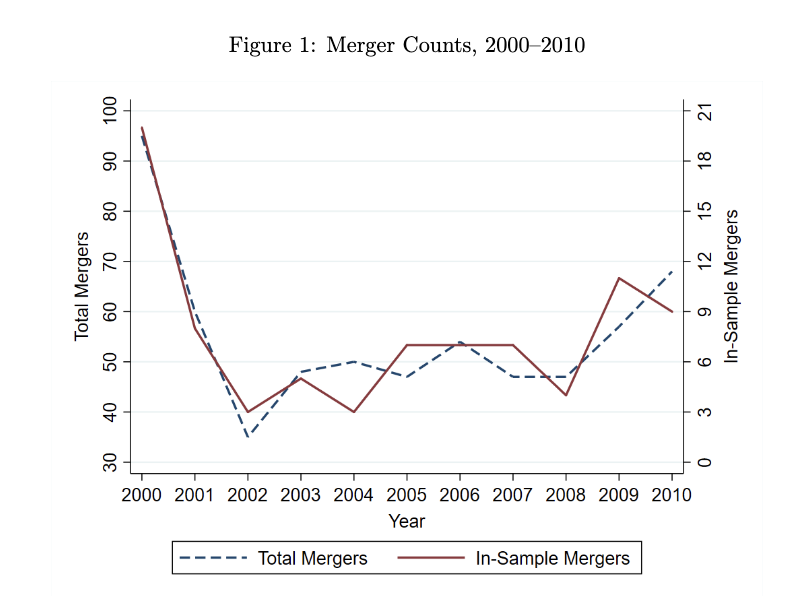
\includegraphics[width=0.6\textwidth]{merger_counts.png}
    \caption{Number of hospital mergers by year (2000-2010)}
  \end{figure}
\end{frame}

\begin{frame}{Model}
  \begin{equation}
    ln(wage_{imt}) = \delta_i + \tau_t + \alpha \textcolor{red}{post_{mt}} + X_{imt}\beta + \epsilon_{imt}
  \end{equation}
\end{frame}

\begin{frame}{Parallel Trends Check}
  \begin{figure}
    \centering
    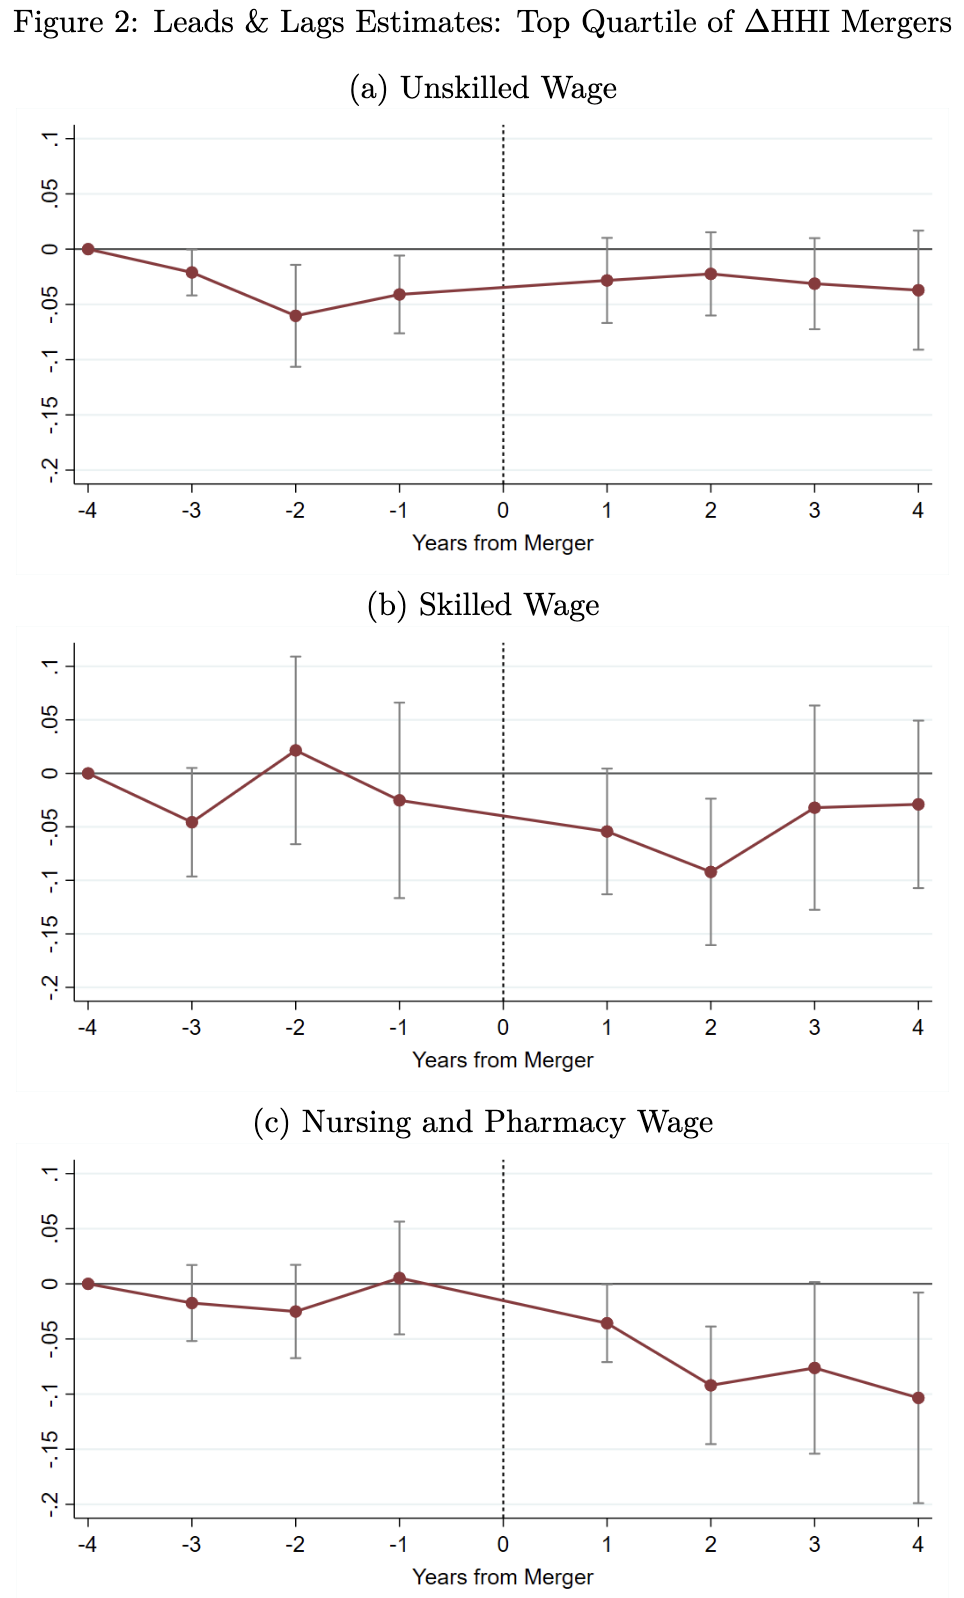
\includegraphics[width=0.33\textwidth]{parallel_trends.png}
    \caption{Wage trend differences (top quartile of concentration)}
  \end{figure}
\end{frame}

% Section 3
\section{Results}


\begin{frame}{Difference-in-Differences Estimates}
\scriptsize
\setlength{\tabcolsep}{4pt}
\renewcommand{\arraystretch}{0.9}
  \begin{centering}

    \begin{tabular}{lccc}
    \toprule
    & (1) & (2) & (3) \\
    & Unskilled & Skilled & Nursing \& Pharmacy \\
    \midrule
    Post & 0.005 & -0.006 & -0.007 \\
        & (0.005) & (0.008) & (0.006) \\
    \addlinespace
    Observations & 17,458 & 17,453 & 17,328 \\
    R-squared    & 0.913  & 0.852  & 0.875  \\
    \midrule
    & (4) & (5) & (6) \\
    & Unskilled & Skilled & Nursing \& Pharmacy \\
    \midrule
    Post $\times$ 1st quartile $\Delta$HHI & 0.004 & 0.005 & 0.002 \\
                                          & (0.006) & (0.010) & (0.009) \\
    Post $\times$ 2nd quartile $\Delta$HHI & 0.007 & -0.022 & -0.001 \\
                                          & (0.009) & (0.016) & (0.010) \\
    Post $\times$ 3rd quartile $\Delta$HHI & 0.007 & 0.002 & -0.019 \\
                                          & (0.008) & (0.021) & (0.014) \\
    Post $\times$ 4th quartile $\Delta$HHI & 0.002 & -0.041** & -0.070*** \\
                                          & (0.014) & (0.019) & (0.022) \\
    \addlinespace
    Observations & 17,458 & 17,453 & 17,328 \\
    R-squared    & 0.913  & 0.853  & 0.875  \\
    \midrule
    $H_{0}$: no heterogeneity & 0.978 & 0.105 & 0.016** \\
    \bottomrule
    \end{tabular}

  \end{centering}
\end{frame}

\begin{frame}{Hospital Employer Concentration in Main Merger Sample}
\centering

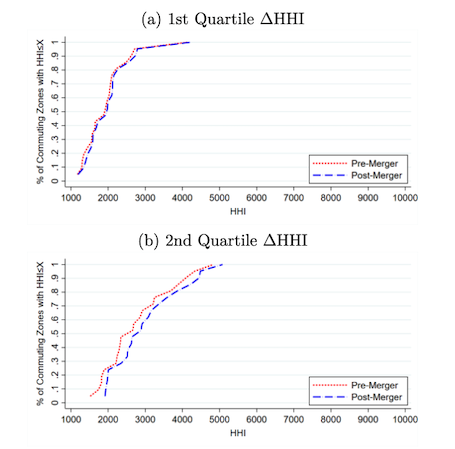
\includegraphics[width=\linewidth,
                 height=0.85\textheight,
                 keepaspectratio]{hhi_cdf12}
\end{frame}

\begin{frame}{Hospital Employer Concentration in Main Merger Sample}
\centering

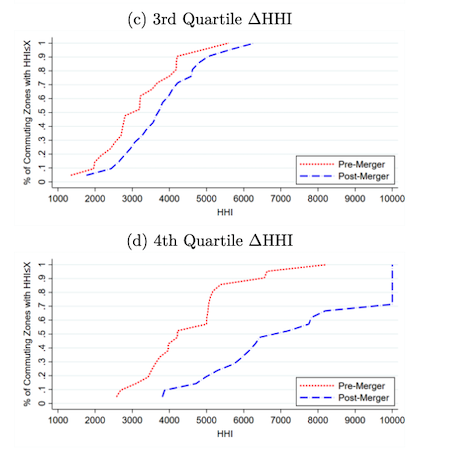
\includegraphics[width=\linewidth,
                 height=0.85\textheight,
                 keepaspectratio]{hhi_cdf34}
\end{frame}

\begin{frame}{Heat Map of HHI Concentration (2012)}
  \centering
  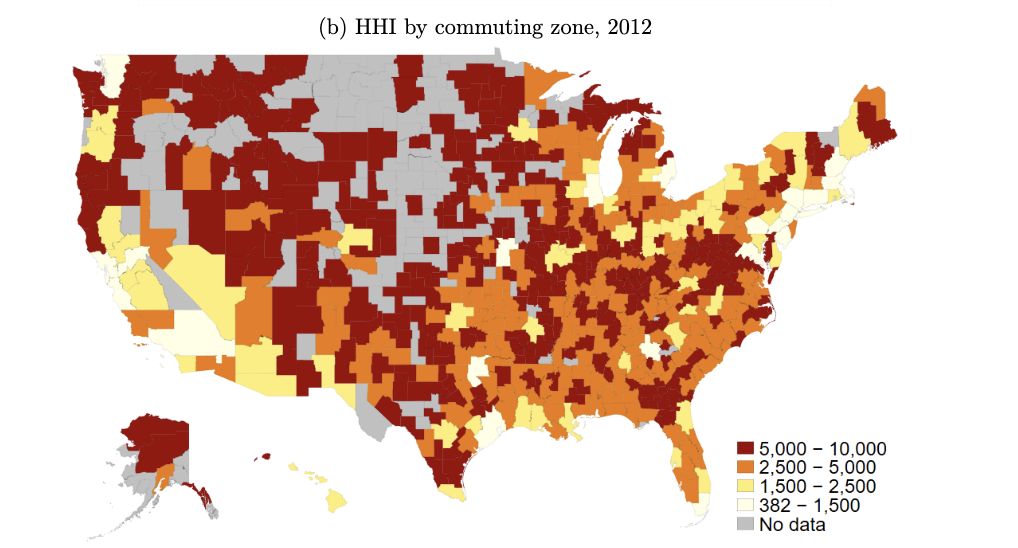
\includegraphics[width=0.8\linewidth,
                   height=0.8\textheight,
                   keepaspectratio]{hhi_concentration.png}
\end{frame}

\begin{frame}{Cohort-by-Cohort Estimation}
\scriptsize
\setlength{\tabcolsep}{5pt}
\renewcommand{\arraystretch}{0.9}

\begin{tabular}{lcc}
\toprule
& (1) & (2) \\
& Main Text & Wgt. Avg. of Cohort-by-Cohort \\
\midrule
\textit{Unskilled:} & & \\
Post $\times$ 1st quartile $\Delta$HHI & 0.004 & 0.004 \\
Post $\times$ 2nd quartile $\Delta$HHI & 0.007 & 0.007 \\
Post $\times$ 3rd quartile $\Delta$HHI & 0.007 & 0.007 \\
Post $\times$ 4th quartile $\Delta$HHI & 0.002 & 0.001 \\
\addlinespace
\textit{Skilled:} & & \\
Post $\times$ 1st quartile $\Delta$HHI & 0.005 & 0.002 \\
Post $\times$ 2nd quartile $\Delta$HHI & -0.022 & -0.022 \\
Post $\times$ 3rd quartile $\Delta$HHI & 0.002 & 0.003 \\
Post $\times$ 4th quartile $\Delta$HHI & -0.041 & -0.040 \\
\addlinespace
\textit{Nursing \& Pharmacy:} & & \\
Post $\times$ 1st quartile $\Delta$HHI & 0.002 & 0.002 \\
Post $\times$ 2nd quartile $\Delta$HHI & -0.001 & -0.001 \\
Post $\times$ 3rd quartile $\Delta$HHI & -0.019 & -0.018 \\
Post $\times$ 4th quartile $\Delta$HHI & -0.070 & -0.067 \\
\bottomrule
\end{tabular}

\medskip
\tiny\emph{Notes:} Column (1) repeats the point estimates from the baseline regressions (equation (1) / Table 3). Column (2) reports weighted averages of cohort-specific estimates (Goodman-Bacon 2019; Callaway \& Sant’Anna 2019).
\end{frame}

\section{Counterfactual Estimations}
\begin{frame}{Counterfactuals}
  \begin{itemize}
    \item Counterfactual 1: Out-of-market mergers
    \begin{itemize}
      \item shifts in instutitutional properties of hospitals influence wages
      \item ambiguous findings, no significant deviation from main results
    \end{itemize}
    \item Counterfactual 2: Non-wage compensation
    \begin{itemize}
      \item CMS Wage Index Files - spending on hospital services would need to rise by 200+ percent to explain wage reductions
    \end{itemize}
    \item Counterfactual 3: Labor unions
    \begin{itemize}
      \item high unionization rates meaningfully attenuate wage growth reductions post-merger
    \end{itemize}
    \item Counterfactual 4: Monoposony
    \begin{itemize}
      \item No evidence of reductions in employment growth
      \item nursing and pharmacy cohort sees \textit{faster} growth in employment in treated markets
    \end{itemize}
  \end{itemize}
\end{frame}

\begin{frame}{Out-of-Market Mergers}
\scriptsize
\setlength{\tabcolsep}{4pt}
\renewcommand{\arraystretch}{0.9}

\begin{tabular}{lccc}
\toprule
& (1) & (2) & (3) \\
& Unskilled & Skilled & Nursing \& Pharmacy \\
\midrule
Post & 0.002 & -0.010 & 0.004 \\
     & (0.008) & (0.011) & (0.008) \\
\addlinespace
Observations & 15,402 & 15,424 & 15,304 \\
R-squared    & 0.907  & 0.849  & 0.875 \\
\midrule
& (4) & (5) & (6) \\
& Unskilled & Skilled & Nursing \& Pharmacy \\
\midrule
Post $\times$ 1st quartile HHI & 0.008 & -0.005 & -0.005 \\
                               & (0.011) & (0.014) & (0.010) \\
Post $\times$ 2nd quartile HHI & -0.006 & -0.017 & -0.002 \\
                               & (0.010) & (0.017) & (0.012) \\
Post $\times$ 3rd quartile HHI & -0.010 & -0.024 & 0.029 \\
                               & (0.012) & (0.027) & (0.021) \\
Post $\times$ 4th quartile HHI & 0.011 & -0.016 & 0.001 \\
                               & (0.016) & (0.028) & (0.024) \\
\addlinespace
Observations & 15,402 & 15,424 & 15,304 \\
R-squared    & 0.907  & 0.849  & 0.875 \\
\midrule
$H_{0}$: no heterogeneity & 0.566 & 0.901 & 0.566 \\
\bottomrule
\end{tabular}

\medskip
\tiny\emph{Notes:} ***$p<0.01$, **$p<0.05$, *$p<0.10$. Includes hospital/year FE, plus controls (log rent, log population, log beds, log case mix index, \% Medicare, \% Medicaid, \% outpatient charges, log income, \% unemployment, \% age 65+). Errors clustered by hospital; obs. weighted by discharges. Bottom row reports p-value of test of equality across quartiles.
\end{frame}

\begin{frame}{Unionization}
  \begin{figure}
    \centering
    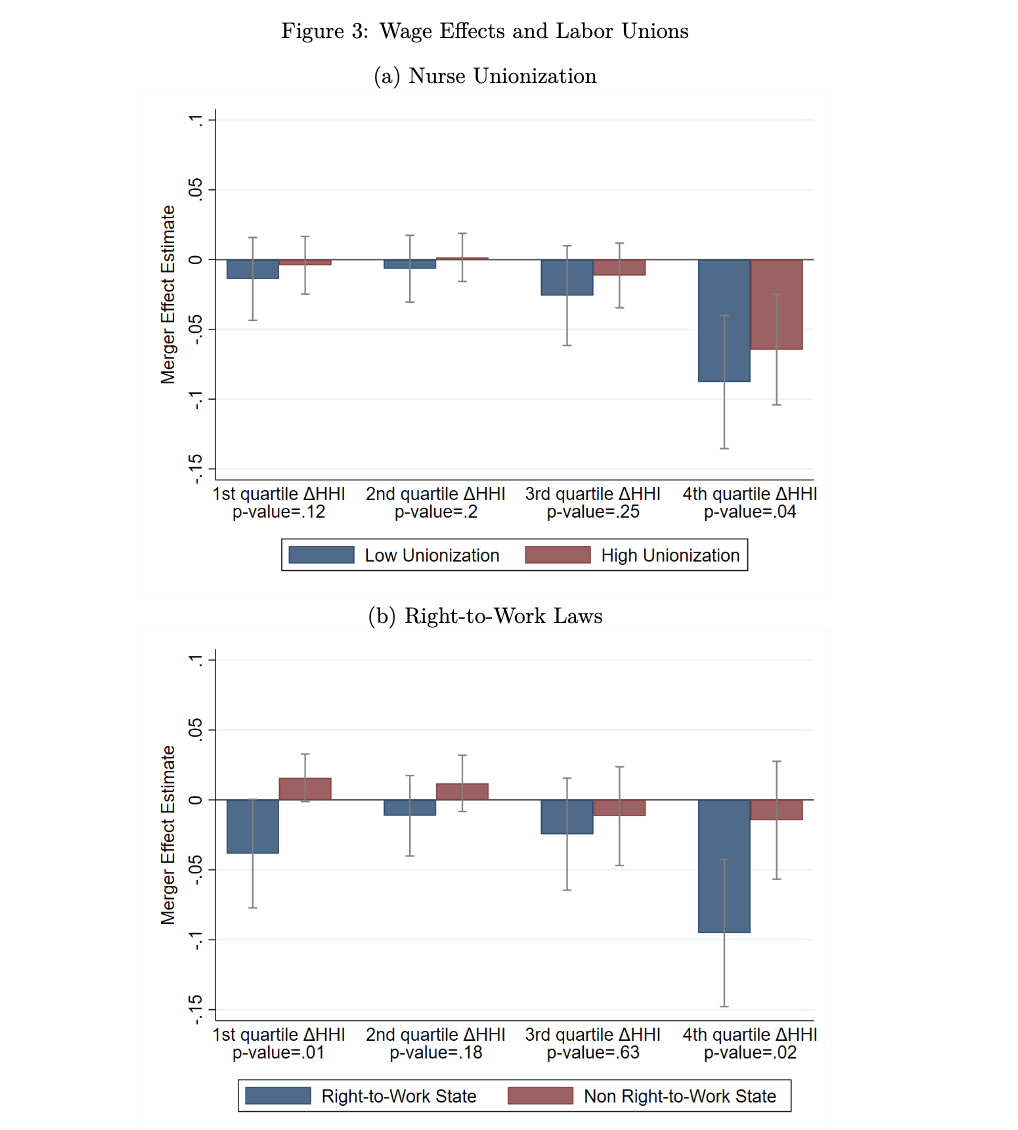
\includegraphics[width=0.6\textwidth]{counterfactual_union.png}
    \caption{Unionization effects on wages}
  \end{figure}
\end{frame}

\begin{frame}{Monopsony}
\scriptsize
\setlength{\tabcolsep}{4pt}
\renewcommand{\arraystretch}{0.3}

\textbf{Panel A: Labor Quantity (log FTEs)}

\begin{tabular}{lccc}
\toprule
& (1) & (2) & (3) \\
& Unskilled & Skilled & Nursing \& Pharmacy \\
\midrule
Post $\times$ 1st quartile $\Delta$HHI & -0.006 & 0.024 & -0.033 \\
                                       & (0.021) & (0.025) & (0.030) \\
Post $\times$ 2nd quartile $\Delta$HHI & -0.011 & 0.060* & -0.081 \\
                                       & (0.032) & (0.036) & (0.056) \\
Post $\times$ 3rd quartile $\Delta$HHI & -0.002 & -0.020 & 0.078 \\
                                       & (0.022) & (0.055) & (0.061) \\
Post $\times$ 4th quartile $\Delta$HHI & 0.045 & -0.046 & 0.187** \\
                                       & (0.051) & (0.075) & (0.081) \\
\addlinespace
Observations & 18,079 & 18,067 & 17,885 \\
R-squared    & 0.959  & 0.913  & 0.923 \\
\bottomrule
\end{tabular}

\medskip
\textbf{Panel B: Labor Composition (Nursing)}

\begin{tabular}{lccc}
\toprule
& (4) & (5) & (6) \\
& (log) RN FTEs & (log) LPN FTEs & LPN Share \\
\midrule
Post $\times$ 1st quartile $\Delta$HHI & 0.007 & -0.148** & 0.001 \\
                                       & (0.015) & (0.062) & (0.003) \\
Post $\times$ 2nd quartile $\Delta$HHI & -0.001 & 0.038 & -0.001 \\
                                       & (0.022) & (0.052) & (0.004) \\
Post $\times$ 3rd quartile $\Delta$HHI & 0.020 & 0.009 & -0.005 \\
                                       & (0.041) & (0.079) & (0.005) \\
Post $\times$ 4th quartile $\Delta$HHI & 0.074 & 0.042 & -0.005 \\
                                       & (0.065) & (0.133) & (0.007) \\
\addlinespace
Observations & 17,575 & 17,299 & 17,576 \\
R-squared    & 0.975  & 0.819  & 0.854 \\
\bottomrule
\end{tabular}

\medskip
\tiny\emph{Notes:} ***$p<0.01$, **$p<0.05$, *$p<0.10$. All specifications include hospital and year fixed effects, plus controls (log rent, log population, log beds, log case mix index, \% Medicare, \% Medicaid, \% outpatient charges, log income, \% unemployment, \% age 65+). Errors clustered by hospital; obs. weighted by discharges.
\end{frame}

% Section 4
\section{Conclusion}

\begin{frame}{Conclusion}
  \begin{itemize}
    \item Wage slowdown found for industry-specific workers, particu8larly in markets with large increases in concentration
    \item Increased labor market power \textit{can} reduce wage growth, though in more defined circumstances than results would suggest
    \item Merger analysis should be sensitive to merger characteristics, worker types, and labor market definitions 
    \item High-skilled workers face harsher penalties in this context due to less competition for their labor
  \end{itemize}
\end{frame}

\end{document}
